% Please use the skeleton file you have received in the 
% invitation-to-submit email, where your data are already
% filled in. Otherwise please make sure you insert your 
% data according to the instructions in PoSauthmanual.pdf

% JRP added to avoid ifpdf name clash in TexShop
\RequirePackage{ifpdf}
%%% END JRP

\documentclass{PoS}

%JRP added
%Uncomment next line if AMS fonts required
 \usepackage{graphicx}
 \usepackage{epstopdf}

 %%% END JRP

\title{Cosmology from EoR/Cosmic Dawn}

\ShortTitle{EoR/CD Cosmology}

\author{\speaker{Pritchard}\thanks{A footnote may follow.}, Chang, Furlanetto, Choudhury, Zaroubi, Santos, Chen, Weller, Abdalla, Mesinger, Metcalf on behalf of the Cosmology-SWG and EoR/CD-SWG\\
        Imperial College London\\
        E-mail: \email{j.pritchard@imperial.ac.uk}}

%\author{Another Author\\
%        Affiliation\\
%        E-mail: \email{...}}

\abstract{SKA Phase 1 will build upon early detections of the EoR by precursor instruments, such as MWA, PAPER, LOFAR, and HERA, to make the first high signal-to-noise measurements of fluctuations in the 21 cm brightness temperature from both reionization and the cosmic dawn. This will allow both imaging and statistical maps of the 21cm signal at redshifts $z=6-30$ and constrain the underlying cosmology and evolution of the density field. This era includes nearly 60\% of the (in principle) observable volume of the Universe and many more linear modes than the CMB, presenting an opportunity for SKA to usher in a new level of precision cosmology. This optimistic picture is complicated by the need to understand and remove the effect of astrophysics, so that systematics rather than statistics will limit constraints.

This chapter will describe the cosmological, as opposed to astrophysical, information available to SKA Phase 1. Key areas for discussion include: cosmological parameters constraints using 21cm fluctuations as a tracer of the density field; lensing of the 21cm signal, constraints on heating via exotic physics such as decaying or annihilating dark matter; impact of fundamental physics such as non-Gaussianity or warm dark matter on the source population; and constraints on the bulk flows arising from the decoupling of baryons and photons at $z=1000$. The chapter will explore the path to separating cosmology from `gastrophysics', for example via velocity space distortions and separation in redshift. We will discuss new opportunities for extracting cosmology made possible by the sensitivity of SKA-1 and explore the advances achievable with SKA-2.
}

\FullConference{
Advancing Astrophysics with the Square Kilometre Array\\
June 8-13, 2014\\
Giardini Naxos, Italy}

%Add new definitions here
%user defined shortcuts
%Journal definitions
\newcommand{\apj}{ApJ}
\newcommand{\apjl}{ApJ}
\newcommand{\apjs}{ApJS}
\newcommand{\aap}{A \& A}
\newcommand{\aj}{AJ}
\newcommand{\araa}{ARAA}
\newcommand{\mnras}{MNRAS}
\newcommand{\physrep}{Phys. Rep.}
\newcommand{\prd}{PRD}
\newcommand{\nat}{Nat.}
\newcommand{\jcap}{JCAP}
\newcommand{\sovast}{Sov. Astron.}
\newcommand{\nar}{New Astron. Rev.}
\newcommand{\apss}{Astrophys. \& Space. Sci.}

\newcommand{\ud}{{\rm d}}

%%%% END NEW DEFINITIONS

\begin{document}

%%%%%%%%%%%%%%%%%%%%%%%%%%%%%
%%%%%%%%%%%%%%%%%%%%%%%%%%%%%
\section{Introduction}

The years since the COBE observations of the CMB have ushered in an age of precision cosmology. Key cosmological parameters have been made possible by measurements of the distribution of matter in the Universe through WMAP and Planck observations of CMB anisotropies and large volume galaxy surveys such as SDSS. These surveys have made precision measurements of parameters describing the matter content of the Universe - the baryons $\Omega_b$, dark matter $\Omega_c$, dark energy $\Omega_\Lambda$, radiation $\Omega_r$, and neutrinos $\Omega_\nu$ - and the physics of inflation - via the tilt $n_s$, amplitude $A_s$, running $\ud n_s/\ud\log k$ or the primordial potential power spectrum and $r$ the ratio of tensor-to-scalar modes produced by inflation. These measurements have firmly established the basic picture of our Universe, known widely as the $\Lambda$CDM model of cosmology.

Despite this progress, measuring these numbers is only the first step towards a deep understanding of the underlying physics. Our ignorance of the nature of the dark matter and the dark energy or how neutrinos acquire mass and what value that mass takes are just two questions that modern cosmology hopes to address. Over the next decade two paths will help shed light on this. The simplest is simply to measure these cosmological parameters ever more precisely and over a wider range of times and scales in the hope of gaining further insights. The exemplar of this is with dark energy, where attempts to measure the redshift evolution of the dark energy density, parameterised by an equation of state $w(z)$, might distinguish a true cosmological constant from more general dark energy or modified gravity. For others there are critical thresholds of precision required to distinguish physical scenarios - for example, measuring the sum of the neutrino masses $M_\nu\lesssim0.1$ would determine the neutrino mass hierarchy. Clearly more precision is a good thing, but it is not the only path forward.

Secondly, we can seek signatures of new physics in ways distinct from the distribution of large scale matter. The processes that produce dark matter will also allow it to annihilate and maybe to decay. The release of energy might have impact on the surrounding environment, heating the intergalactic medium. Pursuing unique signatures of new physics in new regimes will be a key part of the next decade.

The SKA is uniquely placed to probe cosmology as it is capable of mapping the Universe over wide volumes and an unprecedented range of redshifts. Figure \ref{fig:volume} illustrates the additional range of volume and redshifts that the SKA will constrain. In this chapter, we will focus on the new opportunities created by SKA observations of the epoch of reionization (EoR) and the cosmic dawn (CD). This period has never before been observed offering a unique opportunity to test the consistency of the $\Lambda$CDM model and search for new hints to the great unanswered questions of cosmology.

\begin{figure}[htbp]
\begin{center}
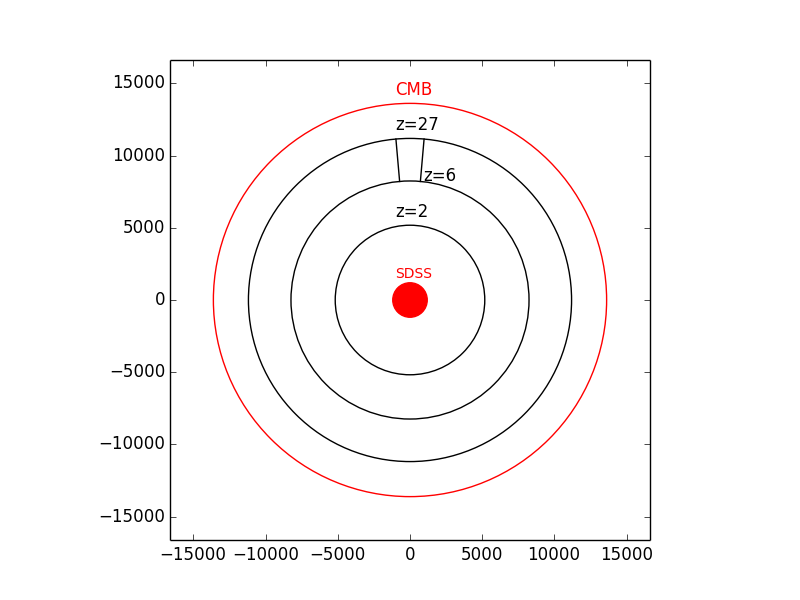
\includegraphics[scale=0.6]{figures/plotcircles.png}
\caption{Illustration of the volume probed by SKA}
\label{fig:volume}
\end{center}
\end{figure}

\cite{furlanetto2006dm}

%%%%%%%%%%%%%%%%%%%%%%%%%%%%%
%%%%%%%%%%%%%%%%%%%%%%%%%%%%%
\section{Cosmological parameters from density fluctuations}

{\bf Introduce fisher matrix formalism}

In this section, we explore the ability of SKA to constrain cosmological parameters via observations of the density field. Just as galaxy surveys constrain cosmology by using galaxies as a tracer of the linear density field, SKA can constrain cosmology by using the 21 cm brightness temperature as a tracer of the density field. This is not an unproblematic assertion, since brightness temperature fluctuations may be sourced by variation in the spin temperature and neutral fraction in addition to the density field. 

\begin{equation}\label{deltatb}
\delta T_B=(1+\delta)x_H...
\end{equation}
Equation \ref{deltatb} shows how these different terms come into play. In a regime where $T_S\gg T_{\rm CMB}$ and $x_H=1$ then $\delta T_B$ will be an unbiased tracer of the density field. At all other times the effects of astrophysics must be modelled and removed or somehow avoided. We will return to a discussion of this point in \S\ref{sec:separation} as this is a critical point.

In this section, we take the optimistic view that there will a regime in which $\delta T_b\propto(1+\delta)$ so that the 21cm signal provides a clean measurement of the density field. This approach enables us to evaluate the best case scenario for SKA in measuring cosmological parameters. By comparing this to galaxy surveys we get a sense of how competitive SKA could be, if astrophysics could be overcome.

The sensitivity of a radio interferometer to the 21cm power spectrum has been well studied \cite{bowman2005, mcquinn2006,mao20??} and we follow the same approach here. The variance of a 21 cm power spectrum estimate for a single
$\mathbf{k}$-mode with line of sight component $k_{||}=\mu k$ is given by
\cite{lidz2007}:
\begin{equation}
\sigma_P^2(k,\mu)= \frac{1}{N_{\rm field}}\left[\bar{T}_b^2P_{21}(k,\mu)+T_{\rm sys}^2\frac{1}{B t_{\rm int}}\frac{D^2\Delta D}{n(k_\perp)}\left(\frac{\lambda^2}{A_e}\right)^2\right]^2.
\end{equation}

The first term on the right-hand-side
of the above expression provides the contribution from sample variance,
while the second describes the thermal noise of the radio telescope.  The
thermal noise depends upon the system temperature $T_{\rm sys}$, the survey
bandwidth $B$, the total observing time $t_{\rm int}$, the conformal
distance $D(z)$ to the center of the survey at redshift $z$, the depth of
the survey $\Delta D$, the observed wavelength $\lambda$, and the effective
collecting area of each antennae tile $A_e$.  The effect of the
configuration of the antennae is encoded in the number density of baselines
$n_\perp(k)$ that observe a mode with transverse wavenumber $k_\perp$
\cite{mcquinn2005}.  Observing a number of fields $N_{\rm field}$ further reduces the variance.

Estimates of the error on a power spectrum measurement are calculated using the Fisher matrix formalism, so that the $1-\sigma$ errors on the model parameter $\lambda_i$ are $(\mathbf{F}_{ij}^{-1})^{1/2}$, where 
\begin{equation}
F_{ij}=\sum_{\rm \mu} \frac{\epsilon k^3 V_{\rm survey}}{4\pi^2}\frac{1}{\sigma_P^2(k,\mu)}\frac{\partial P_{T_b}}{\partial \lambda_i}\frac{\partial P_{T_b}}{\partial \lambda_j}.
\end{equation}
In this equation, $V_{\rm survey}=D^2\Delta D(\lambda^2/A_e)$ denotes the
effective survey volume of our radio telescopes and we assume wavenumber
bins of width $\Delta k=\epsilon k$.  We will be interested in the cases
where $\lambda_i=\{\bar{P}_{T_b}\}$ and $\lambda_i=\{
P_{\mu^0},\,P_{\mu^2},\,P_{\mu^4}\}$.

{\bf sensitivity plot for various experiments relative to density field}

\begin{table}[htdp]
\caption{Low-frequency radio telescopes and their parameters.  We specify the number of antennae $N_a$, total collecting area $A_{\rm tot}$, bandwidth $B$, and total integration time $t_{\rm int}$ for each instrument. These values are fixed at $z=??$ and extrapolated to other frequencies using $A_{\rm tot}=N_{\rm ant}N_{\rm dip}A_{\rm dip}$ with the number of antennae per station $N_{\rm dip}=289$ and $A_{\rm dip}=\min(\lambda^2/3,3.2\,{ \rm m^2})$.}
\begin{center}
\begin{tabular}{ccccccc}
\hline
\hline
Array & $N_a$ & $A_{\rm tot}(10^3\,{\rm m^2})$ & $B$ (MHz) & $t_{\rm int}$ (hr)& $R_{\rm min} (m)$ & $R_{\rm max} (km)$\\
\hline
MWA & 112 & 1.6  & 8 & 1000 & 4 & 0.75\\
LOFAR Core & 48 & 38.6  & 8 & 1000 & 100 & 1.5\\
HERA & 331 & 50.0  & 8 & 1000 & 14.3 & 0.3\\
SKA0 & 650$\times$0.5 & 224$\times$0.5  & 8 & 1000 & 35 & 1\\
SKA1 & 650 & 224  & 8 & 1000 & 35 & 1\\
SKA2 & 650$\times$4 & 224$\times$4 & 8 & 1000 & 35 & 1\\
\hline
\hline
\end{tabular}
\end{center}
\label{tab:telescopes}
\end{table}%

We first illustrate the sensitivity of different iterations of SKA in Figure \ref{fig:sensitivity}, where we take the parameters in Table \ref{tab:telescopes} for SKA0 - with 50\% of the SKA1 baseline collecting area, SKA1, and SKA2 - with x4 the collecting area of SKA1. For each of these we assume a filled core of radius $R_{\max}$ and ignore all antennae outside this distance. 

{\bf SKA1 has 911 stations total with 899 in the core and 650 stations within a radius of 1km accounting for ~75\% of the total number of stations and collecting area. Physical station size is 35m. Stations have 289 antennae with antennae area $A_e=\lambda^2/3$ giving $3.2m^2$ at 110MHz. At lower frequencies the array is densely packed and has constant collecting area, at higher frequencies the array becomes sparse.}

\begin{figure}[htbp]
\begin{center}
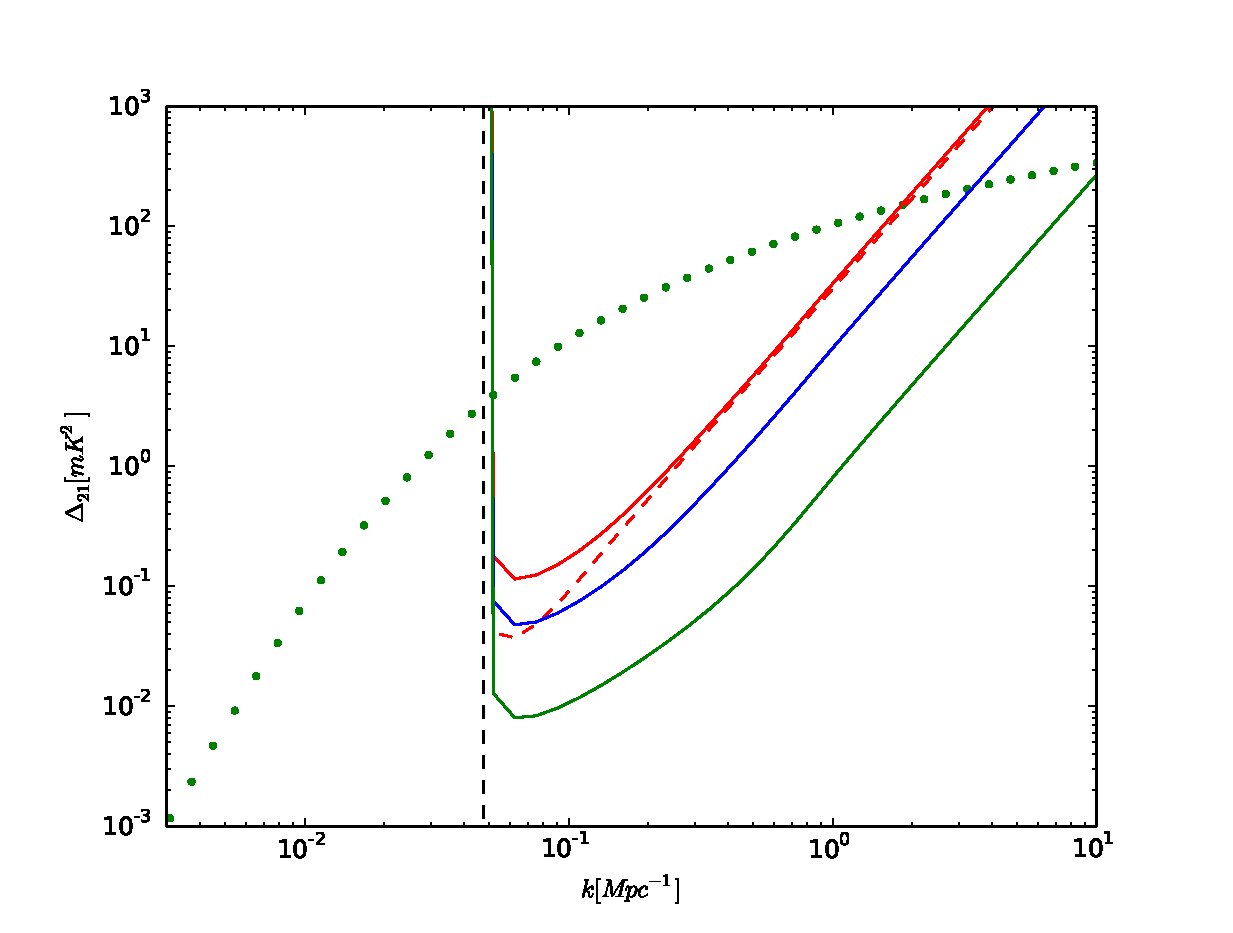
\includegraphics[scale=0.35]{figures/sensitivityPlot_z8.eps}
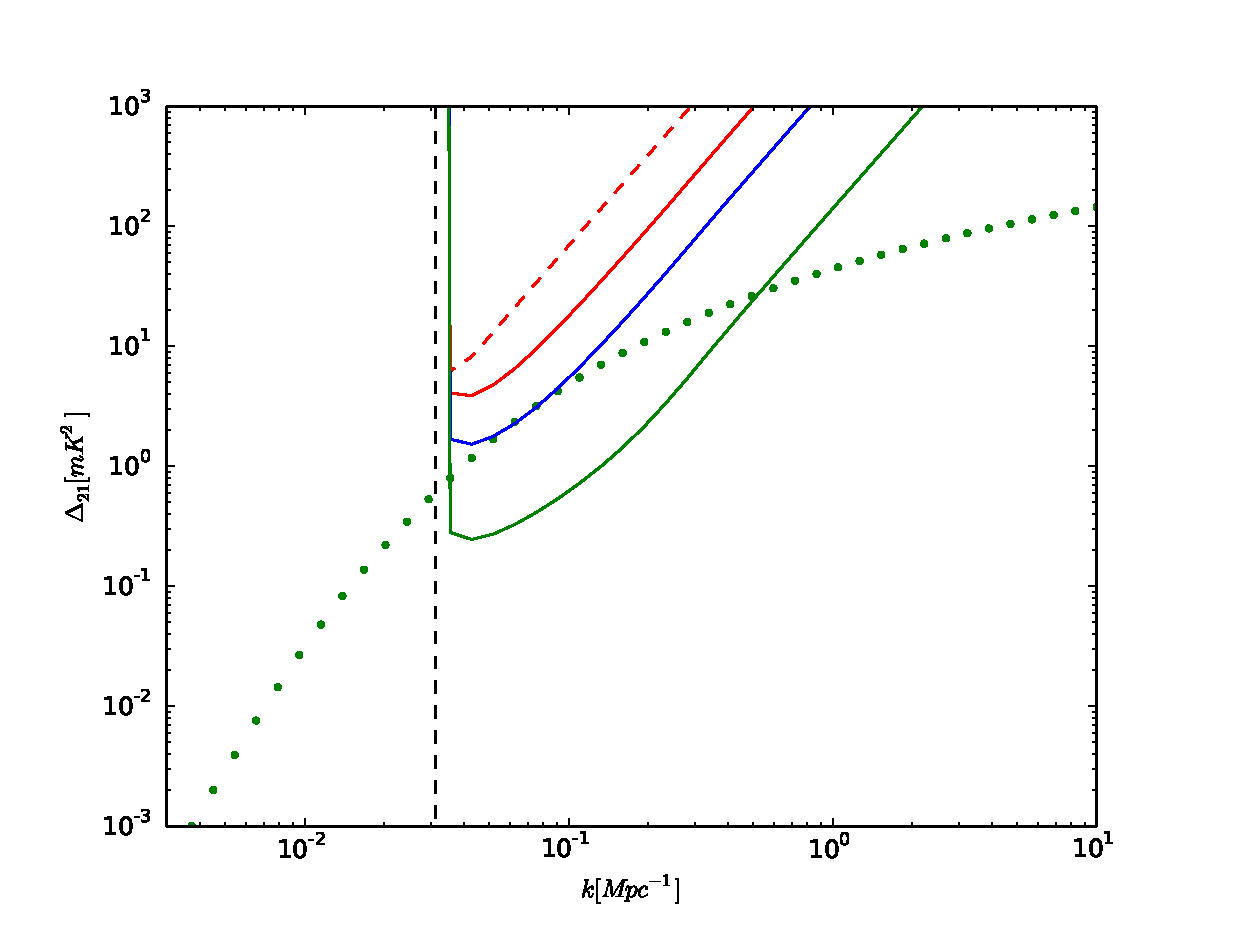
\includegraphics[scale=0.35]{figures/sensitivityPlot_z20.eps}
\caption{Sensitivity plots of HERA (red dashed curve), SKA0 (red), SKA1 (blue), and SKA2 (green). Dotted curve shows the predicted 21cm signal from the density field alone assuming $x_H=1$ and $T_S\gg T_{\rm CMB}$. Vertical black dashed line indicates the smallest wavenumber probed in the frequency direction $k=2\pi/y$, which may limit foreground removal.  {\em Left panel:} $z=8$ {\em Right panel:} $z=20$.}
\label{fig:sensitivity}
\end{center}
\end{figure}

Figure \ref{fig:sensitivity} illustrates a few key points governing parameter constraints. The large station sizes remove sensitivity to the largest physical scales (smallest $k$ modes). By $z=20$ the amplitude of the 21 cm signal is too small to be detected by SKA1 {\em if we assume $T_S\gg T_\gamma$}. Detection of the 21cm signal at $z\gtrsim20$ with SKA1 is dependent upon a strong 21cm absorption signal that boosts the amplitude of the 21cm power spectrum. Unfortunately, it seems likely that during the absorption regime the details and spatial variation of the spin temperature will matter and complicated getting at cosmology.

{\bf concept of effective volume and how SKA compares to various galaxy surveys}

The key parameters for determining cosmological parameters are the effective volume probed and the minimum wavenumber probed $k_{\rm min}$ where modes can still be assumed to be linear. SKA has a significant advantage over galaxy surveys as more modes are still in the linear regime at $z>6$. We set $k_{\rm min}=2{\rm Mpc^{-1}}$ {\bf justify or do better}

\begin{figure}[htbp]
\begin{center}

\caption{Effective volume and comparison of SKA to Euclid}
\label{fig:effectivevolume}
\end{center}
\end{figure}

Comment on higher redshift giving other advantages, eg isocurvature, where effects become smaller deeper into matter dominated regime.

Table \ref{tab:constraints} shows the cosmological parameters obtained with the listed experimental performances.

\begin{table*}[htdp]
\caption{Fiducial parameter values and $1-\sigma$ experimental uncertainties for cosmological parameters.  Dashes indicate parameters not relevant for that experiment; $\infty$ indicates parameters that are relevant, but not constrained. }
\begin{center}
\begin{tabular}{c|cccccccc|c}
\hline
& $\Omega_mh^2$ & $\Omega_bh^2$ & $\Omega_\Lambda$ & $w$ & $n_s$ & $A^2_s$ & $\tau$ & $Y_{He}$  & $M_\nu$ \\
\hline
Fiducial& 0.147 & 0.023 & 0.7 & -1 & 0.95 & 26.6 & 0.1 & 0.24 & 0.3  \\
\hline
SDSS& 0.456 & 0.083 & 0.117 & 1.21 & 0.503 & $\infty$ & \ldots & \ldots   \\
\end{tabular}
\end{center}
\label{tab:constraints}
\end{table*}

\subsection{Core cosmological parameters}

\subsection{Inflationary parameters}

\subsection{Neutrino mass}



%%%%%%%%%%%%%%%%%%%%%%%%%%%%%
%%%%%%%%%%%%%%%%%%%%%%%%%%%%%
\section{Constraining new physics from heating}

%%%%%%%%%%%%%%%%%%%%%%%%%%%%%
%%%%%%%%%%%%%%%%%%%%%%%%%%%%%
\section{Fundamental physics from modifications to the source population}

%%%%%%%%%%%%%%%%%%%%%%%%%%%%%
%%%%%%%%%%%%%%%%%%%%%%%%%%%%%
\section{Bulk flows}

%%%%%%%%%%%%%%%%%%%%%%%%%%%%%
%%%%%%%%%%%%%%%%%%%%%%%%%%%%%
\section{Cosmic shear and the EoR}

Ben Metcalf to prepare a summary updated for SKA parameters.

%%%%%%%%%%%%%%%%%%%%%%%%%%%%%
%%%%%%%%%%%%%%%%%%%%%%%%%%%%%
\section{Separating ``gastrophysics" and cosmology}
\label{sec:separation}

%%%%%%%%%%%%%%%%%%%%%%%%%%%%%
%%%%%%%%%%%%%%%%%%%%%%%%%%%%%
\section{Paths to cosmology with Phase 1 and Phase 2}

%%%%%%%%%%%%%%%%%%%%%%%%%%%%%
%%%%%%%%%%%%%%%%%%%%%%%%%%%%%
\section{Miscellaneous?}

%%%%%%%%%%%%%%%%%%%%%%%%%%%%%
%%%%%%%%%%%%%%%%%%%%%%%%%%%%%

%JRP use bibtex while editing
\bibliographystyle{unsrt}
\bibliography{cosmchapterbib}{}
%%% END JRP

%%% Fill copy in .bbl at end
%\begin{thebibliography}{99}
%\bibitem{...}
%\end{thebibliography}
% END COMMENTED OUT BIB

\end{document}
